\documentclass[aspectratio=169,11pt]{beamer}

% ============================================================
% Theme
% ============================================================
\usetheme{Madrid}
\usecolortheme{seahorse}
\setbeamertemplate{navigation symbols}{}


% ============================================================
% Encoding (pdfLaTeX-safe)
% ============================================================
\usepackage[utf8]{inputenc}
\usepackage[T1]{fontenc}
\usepackage{lmodern}

% ============================================================
% Packages
% ============================================================
\usepackage{amsmath,amssymb}
\usepackage{xcolor}
\usepackage{booktabs}
\usepackage{listings}
\usepackage{tikz}
\usetikzlibrary{arrows.meta,positioning,calc,fit}

% ============================================================
% Listings
% ============================================================
\lstset{
	basicstyle=\ttfamily\small,
	frame=single,
	breaklines=true,
	columns=fullflexible,
	showstringspaces=false,
	keywordstyle=\color{blue},
	commentstyle=\color{gray},
	stringstyle=\color{red}
}

% ============================================================
% Title
% ============================================================
\title{Concurrency \& Distributed Systems}
\subtitle{Week 3: Synchronization, Memory Semantics \& Deadlocks\\Day 1 --- Part 2: What \texttt{synchronized} Guarantees and How It Eliminates Races}
\author{Dr. Mohamad Aoude}
\institute{Lebanese University \\ Faculty of Engineering}
\date{}

% ============================================================
% TikZ Styles
% ============================================================
\tikzset{
	box/.style={draw, rounded corners=2pt, align=center, inner sep=6pt},
	smallbox/.style={draw, rounded corners=2pt, align=center, inner sep=3pt},
	arrow/.style={-Latex, line width=0.8pt},
	dashedarrow/.style={-Latex, dashed, line width=0.8pt},
	tinylabel/.style={font=\scriptsize},
	pill/.style={draw, rounded corners=10pt, inner sep=4pt, align=center}
}

\begin{document}
	
	% ============================================================
	% Title slide
	% ============================================================
	\begin{frame}
		\titlepage
	\end{frame}
	
	% ============================================================
	\begin{frame}{A Simple Analogy Before We Begin}
		\begin{block}{Think of a single-key room}
			A \texttt{synchronized} block is like a room with one key:
			\begin{itemize}
				\item only one person can enter at a time
				\item everyone else must wait outside
				\item when the person leaves, the room state is now up to date for the next person
			\end{itemize}
		\end{block}
		
		\bigskip
		
		\begin{alertblock}{Why this analogy helps}
			It captures both ideas:
			\textbf{exclusive access} and \textbf{seeing the latest state}.
		\end{alertblock}
	\end{frame}
	
	% ============================================================
	\begin{frame}{Block 3 --- What \texttt{synchronized} Really Guarantees}
		\begin{block}{This is the conceptual pillar}
			\texttt{synchronized} does \textbf{two} things:
			\begin{itemize}
				\item it provides \textbf{mutual exclusion}
				\item it provides \textbf{visibility guarantees}
			\end{itemize}
		\end{block}
		
		\bigskip
		
		\begin{alertblock}{Key message}
			If students understand only “one thread at a time,” they understand only half of synchronization.
		\end{alertblock}
	\end{frame}
	
	% ============================================================
	\begin{frame}{Guarantee 1 --- Mutual Exclusion}
		\begin{block}{Definition}
			\textbf{Mutual exclusion} means that no two threads execute the same protected critical section at the same time.
		\end{block}
		
		\bigskip
		
		\begin{itemize}
			\item One thread acquires the monitor
			\item Other threads trying to enter become \textbf{BLOCKED}
			\item The protected code runs in an exclusive region
		\end{itemize}
		
		\bigskip
		
		\begin{alertblock}{Why it matters}
			This prevents unsafe interleaving of read--modify--write operations such as \texttt{count++}.
		\end{alertblock}
	\end{frame}
	
	% ============================================================
	\begin{frame}{Guarantee 2 --- Visibility}
		\begin{block}{Definition}
			\textbf{Visibility} means that writes made by one thread become observable to another thread in a well-defined way.
		\end{block}
		
		\bigskip
		
		\begin{itemize}
			\item When a thread exits a synchronized block, its writes are committed so other threads can observe them
			\item When another thread later enters a synchronized block guarded by the same monitor, it sees fresh values
		\end{itemize}
		
		\bigskip
		
		\begin{alertblock}{Important}
			\texttt{synchronized} is not only about “keeping threads apart.”  
			It also governs what values threads are allowed to see.
		\end{alertblock}
	\end{frame}
	
	% ============================================================
	\begin{frame}{A Simplified Java Memory Model View}
		\begin{block}{Mental model}
			Each thread may work with its own temporary view of memory, while shared variables conceptually live in main memory.
		\end{block}
		
		\bigskip
		
		\centering
		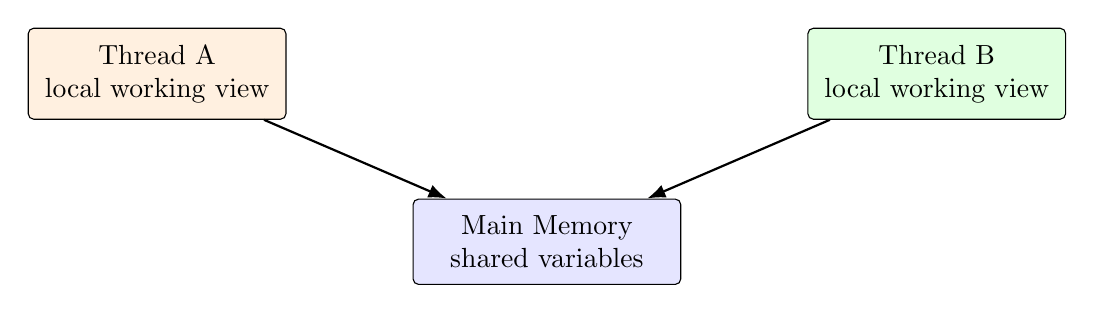
\begin{tikzpicture}[node distance=10mm and 16mm]
			\node[box, fill=blue!10, minimum width=3.4cm] (main) {Main Memory\\shared variables};
			\node[box, fill=orange!12, above left=of main, minimum width=3cm] (t1) {Thread A\\local working view};
			\node[box, fill=green!12, above right=of main, minimum width=3cm] (t2) {Thread B\\local working view};
			
			\draw[arrow] (t1) -- (main);
			\draw[arrow] (t2) -- (main);
		\end{tikzpicture}
		
		\vspace{0.3cm}
		\begin{alertblock}{Why synchronization matters}
			Without proper synchronization, one thread may keep seeing an old value even after another thread has updated it.
		\end{alertblock}
	\end{frame}
	
	% ============================================================
	\begin{frame}{Formal Java Memory Model Rule}
		\begin{block}{Happens-before rule}
			\centering
			\textbf{Unlock of monitor $M$ happens-before subsequent lock of monitor $M$.}
		\end{block}
		
		\bigskip
		
		\begin{itemize}
			\item Thread A exits a synchronized block on monitor $M$
			\item Thread B later enters a synchronized block on the same monitor $M$
			\item Thread B is guaranteed to observe the writes made by Thread A before the unlock
		\end{itemize}
		
		\bigskip
		
		\begin{alertblock}{Interpretation}
			This is not an implementation trick.  
			It is a formal guarantee of the Java Memory Model.
		\end{alertblock}
	\end{frame}
	
	% ============================================================
	\begin{frame}{Mutual Exclusion vs Visibility}
		\centering
		\begin{tabular}{@{}ll@{}}
			\toprule
			\textbf{Concept} & \textbf{Meaning} \\
			\midrule
			Mutual Exclusion & Only one thread inside the critical section \\
			Visibility & Writes become visible to other threads \\
			\bottomrule
		\end{tabular}
		
		\bigskip
		
		\begin{alertblock}{Students must distinguish them}
			A program may avoid overlap yet still have stale reads if visibility is not guaranteed.
		\end{alertblock}
	\end{frame}
	
\begin{frame}{A Simple Timeline of Visibility}
	\centering
	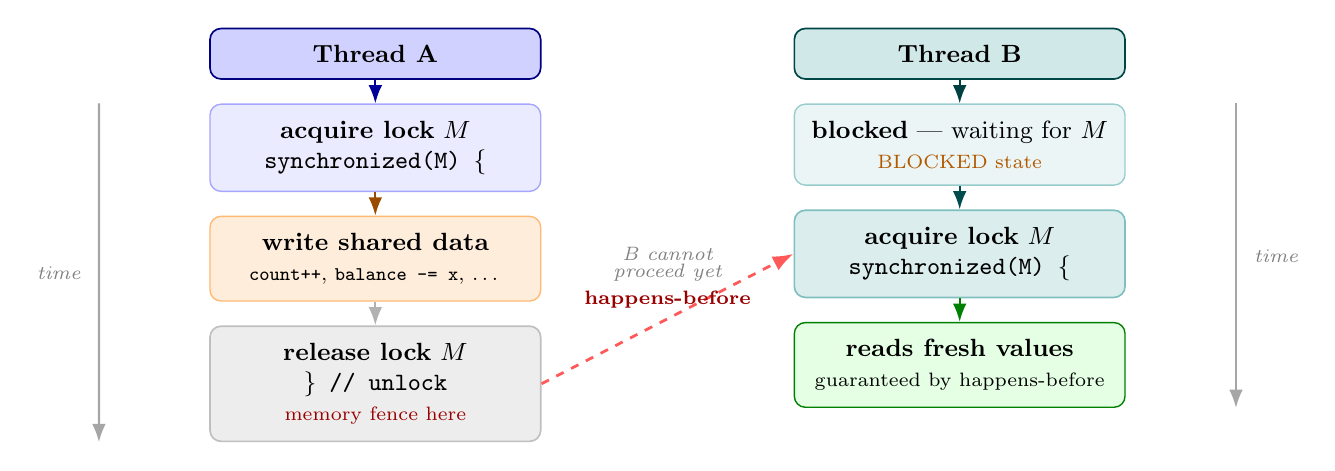
\begin{tikzpicture}[
		stepbox/.style={
			draw, rounded corners=4pt, align=center,
			inner sep=6pt, font=\small
		}
		]
		
		%% -- Thread A column header
		\node[stepbox, fill=blue!18, draw=blue!50!black, line width=0.6pt,
		minimum width=4.2cm, font=\small\bfseries] (ah)
		{Thread A};
		
		%% -- Thread A steps
		\node[stepbox, fill=blue!8, draw=blue!35, line width=0.5pt,
		minimum width=4.2cm, below=3mm of ah] (a1)
		{\textbf{acquire lock} \(M\)\\\texttt{synchronized(M) \{}};
		
		\node[stepbox, fill=orange!14, draw=orange!55, line width=0.5pt,
		minimum width=4.2cm, below=3mm of a1] (a2)
		{\textbf{write shared data}\\
			\scriptsize\texttt{count++},\ \texttt{balance -= x},\ \ldots};
		
		\node[stepbox, fill=gray!14, draw=gray!50, line width=0.6pt,
		minimum width=4.2cm, below=3mm of a2] (a3)
		{\textbf{release lock} \(M\)\\\texttt{\} // unlock}\\
			\scriptsize\textcolor{red!60!black}{memory fence here}};
		
		%% -- Thread B column header (right, aligned with Thread A header)
		\node[stepbox, fill=teal!18, draw=teal!55!black, line width=0.6pt,
		minimum width=4.2cm, font=\small\bfseries,
		right=32mm of ah] (bh)
		{Thread B};
		
		%% -- Thread B steps (lower, sequenced after A's unlock)
		\node[stepbox, fill=teal!8, draw=teal!40, line width=0.5pt,
		minimum width=4.2cm, below=3mm of bh] (b1)
		{\textbf{blocked} --- waiting for \(M\)\\
			\scriptsize\textcolor{orange!70!black}{BLOCKED state}};
		
		\node[stepbox, fill=teal!14, draw=teal!50, line width=0.6pt,
		minimum width=4.2cm, below=3mm of b1] (b2)
		{\textbf{acquire lock} \(M\)\\\texttt{synchronized(M) \{}};
		
		\node[stepbox, fill=green!10, draw=green!50!black, line width=0.5pt,
		minimum width=4.2cm, below=3mm of b2] (b3)
		{\textbf{reads fresh values}\\
			\scriptsize guaranteed by happens-before};
		
		%% -- Thread A flow arrows
		\draw[arrow, blue!60!black]  (ah) -- (a1);
		\draw[arrow, orange!60!black] (a1) -- (a2);
		\draw[arrow, gray!60]         (a2) -- (a3);
		
		%% -- Thread B flow arrows
		\draw[arrow, teal!50!black]   (bh) -- (b1);
		\draw[arrow, teal!60!black]   (b1) -- (b2);
		\draw[arrow, green!50!black]  (b2) -- (b3);
		
		%% -- happens-before arrow from A's unlock to B's acquire
		\draw[dashedarrow, red!65, line width=1.0pt]
		(a3.east) -- (b2.west)
		node[midway, above, font=\scriptsize\bfseries,
		text=red!60!black] {happens-before};
		
		%% -- Time axes
		\draw[-Latex, gray!70, line width=0.8pt]
		([xshift=-14mm] a1.north west) -- ([xshift=-14mm] a3.south west)
		node[midway, left=1mm, font=\scriptsize\itshape, text=gray] {time};
		
		\draw[-Latex, gray!70, line width=0.8pt]
		([xshift=14mm] b1.north east) -- ([xshift=14mm] b3.south east)
		node[midway, right=1mm, font=\scriptsize\itshape, text=gray] {time};
		
		%% -- Sequencing annotation: B cannot proceed until A unlocks
		\node[font=\scriptsize\itshape, text=gray, align=center]
		at ($(a3.east)!0.5!(b1.west)$)
		{B cannot\\[-2pt]proceed yet};
		
	\end{tikzpicture}
	
	\vspace{0.2cm}
	\begin{block}{Core idea}
		The unlock is not just a release of the lock.
		It is a \textbf{memory-ordering event} --- all of Thread A's writes
		become visible to Thread B when B subsequently acquires the same monitor.
	\end{block}
	
\end{frame}
	
	% ============================================================
	\begin{frame}{Common Mistake}
		\begin{alertblock}{Wrong mental model}
			“\texttt{synchronized} only prevents two threads from running together.”
		\end{alertblock}
		
		\bigskip
		
		\begin{block}{Correct mental model}
			\texttt{synchronized} provides:
			\begin{itemize}
				\item exclusive entry into a critical section
				\item visibility of prior writes across threads
			\end{itemize}
		\end{block}
		
		\bigskip
		
		\centering
		\Large Mutual exclusion \(\neq\) visibility
	\end{frame}
	
	% ============================================================
	\begin{frame}{Check Your Understanding}
		\begin{block}{Question}
			If two threads never execute a critical section at the same time, does that automatically mean they always see the latest shared values?
		\end{block}
		
		\bigskip
		
		\begin{enumerate}
			\item Yes, always
			\item No, not unless visibility is also guaranteed
			\item Yes, because exclusion and visibility are the same thing
		\end{enumerate}
		
		\bigskip
		
		\begin{alertblock}{Expected answer}
			\textbf{2}. Preventing overlap is not the same as guaranteeing fresh reads.
		\end{alertblock}
	\end{frame}
	
	% ============================================================
	\begin{frame}{Reentrancy Note}
		\begin{block}{Important property}
			Java intrinsic locks are \textbf{reentrant}.
		\end{block}
		
		\bigskip
		
		\begin{itemize}
			\item If a thread already holds a monitor, it can enter another synchronized section guarded by the same monitor
			\item The same thread does not block itself on the same lock
		\end{itemize}
		
		\bigskip
		
		\begin{alertblock}{Why mention this now?}
			This prevents confusion later when synchronized methods call other synchronized methods on the same object.
		\end{alertblock}
	\end{frame}
	
	% ============================================================
	\begin{frame}{Block 4 --- Fixing the Counter Properly}
		\begin{block}{Goal}
			We now repair the counter using a \textbf{shared lock object}.
		\end{block}
		
		\bigskip
		
		\begin{itemize}
			\item Before: unsynchronized increment
			\item After: protected critical section
		\end{itemize}
		
		\bigskip
		
		\begin{alertblock}{Question}
			What exactly does the fix eliminate?
		\end{alertblock}
	\end{frame}
	
	% ============================================================
	\begin{frame}[fragile]{Counter State with Shared Lock}
		\begin{lstlisting}[language=Java]
			class Counter {
				static int count = 0;
				static final Object lock = new Object();
			}
		\end{lstlisting}
		
		\vspace{0.3cm}
		
		\begin{block}{Design choice}
			The counter is shared, so the lock must also be shared.
		\end{block}
		
		\begin{alertblock}{Why \texttt{final}?}
			The identity of the lock must not change.
		\end{alertblock}
	\end{frame}
	
	% ============================================================
	\begin{frame}[fragile]{Protected Increment}
		\begin{lstlisting}[language=Java]
			synchronized(Counter.lock) {
				Counter.count++;
			}
		\end{lstlisting}
		
		\vspace{0.3cm}
		
		\begin{itemize}
			\item All threads compete for the same monitor
			\item Only one thread increments at a time
			\item Each increment becomes visible to the next thread that acquires the lock
		\end{itemize}
	\end{frame}
	
	% ============================================================
	\begin{frame}{Before vs After Synchronization}
		\centering
		\begin{tabular}{@{}ll@{}}
			\toprule
			\textbf{Before} & \textbf{After} \\
			\midrule
			Lost updates & No lost updates \\
			Unsafe interleaving & Mutual exclusion \\
			No visibility guarantee & Visibility guaranteed \\
			Broken invariant & Race eliminated \\
			\bottomrule
		\end{tabular}
		
		\bigskip
		
		\begin{alertblock}{Key phrase}
			\textbf{Race elimination through synchronization}
		\end{alertblock}
	\end{frame}
	
	% ============================================================
	\begin{frame}{Why the Repair Works}
		\begin{enumerate}
			\item The critical section is now protected by one shared monitor
			\item Read, modify, and write occur without overlap from other threads
			\item Unlock of the monitor makes writes visible
			\item The next thread sees the latest value before incrementing
		\end{enumerate}
		
		\bigskip
		
		\begin{block}{Result}
			The invariant is restored because both interleaving errors and stale observations are controlled.
		\end{block}
	\end{frame}
	
	% ============================================================
	\begin{frame}[fragile]{Spot the Bug}
		\begin{lstlisting}[language=Java]
			void increment() {
				synchronized(new Object()) {
					count++;
				}
			}
		\end{lstlisting}
		
		\vspace{0.3cm}
		
		\begin{alertblock}{What is wrong here?}
			A new lock object is created every time, so threads are \textbf{not} synchronizing on the same monitor.
		\end{alertblock}
		
		\begin{block}{Lesson}
			Synchronization works only when threads contend for the \textbf{same lock object}.
		\end{block}
	\end{frame}
	
	% ============================================================
	\begin{frame}[fragile]{Minimal Runnable Example}
		\begin{lstlisting}[language=Java]
			class Counter {
				static int count = 0;
				static final Object lock = new Object();
				
				static void increment() {
					synchronized(lock) {
						count++;
					}
				}
			}
		\end{lstlisting}
		
		\vspace{0.2cm}
		\begin{alertblock}{Exercise}
			Run the unsynchronized and synchronized versions side by side.
		\end{alertblock}
	\end{frame}
	
	% ============================================================
	\begin{frame}{A Small Preview on Performance}
		\begin{block}{Important trade-off}
			Correct synchronization is necessary, but locking too broadly can reduce concurrency.
		\end{block}
		
		\bigskip
		
		\begin{itemize}
			\item lock too little \(\rightarrow\) unsafe program
			\item lock too much \(\rightarrow\) correct but slower program
		\end{itemize}
		
		\bigskip
		
		\begin{alertblock}{Preview}
			Later we will discuss lock granularity and alternatives such as \texttt{AtomicInteger}.
		\end{alertblock}
	\end{frame}
	
	% ============================================================
	\begin{frame}{Block 5 --- Lab: Bank Account Race}
		\begin{block}{New case study}
			The bug is no longer just a counter mismatch.  
			It is a violation of business logic.
		\end{block}
		
		\bigskip
		
		\begin{alertblock}{Core issue}
			The check and the update must be atomic together.
		\end{alertblock}
	\end{frame}
	
	% ============================================================
	\begin{frame}[fragile]{Unsafe Version}
		\begin{lstlisting}[language=Java]
			public void withdraw(int amount) {
				if (balance >= amount) {
					balance -= amount;
				}
			}
		\end{lstlisting}
		
		\vspace{0.3cm}
		
		\begin{block}{Why unsafe?}
			The condition check and the update are separate actions.
			Another thread may interleave between them.
		\end{block}
	\end{frame}
	
% ============================================================
\begin{frame}{Unsafe Interleaving Example}
	
	\begin{center}
		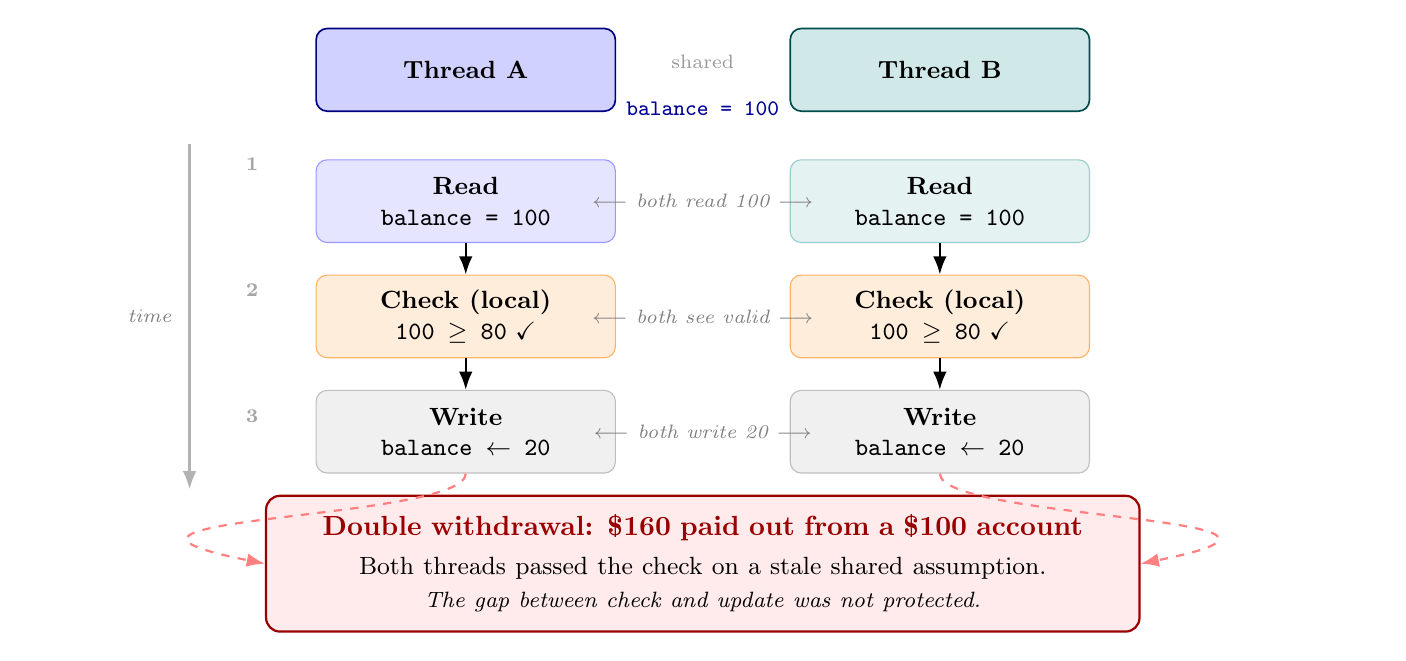
\begin{tikzpicture}[
			stepbox/.style={draw, rounded corners=4pt, align=center,
				inner sep=5pt, minimum width=3.8cm, minimum height=1.05cm,
				font=\small},
			stepnum/.style={font=\scriptsize\bfseries, text=gray!70},
			]
			
			%% -- Column headers
			\node[stepbox, fill=blue!18, draw=blue!50!black, line width=0.6pt,
			font=\small\bfseries] (h1) {Thread A};
			
			\node[stepbox, fill=teal!18, draw=teal!60!black, line width=0.6pt,
			font=\small\bfseries, right=22mm of h1] (h2) {Thread B};
			
			%% -- Step numbers
			\node[stepnum, left=6mm of h1, yshift=-12mm] {1};
			\node[stepnum, left=6mm of h1, yshift=-28mm] {2};
			\node[stepnum, left=6mm of h1, yshift=-44mm] {3};
			
			%% -- STEP 1: Both read
			\node[stepbox, fill=blue!10, draw=blue!40,
			below=6mm of h1] (a1)
			{\textbf{Read}\\\texttt{balance = 100}};
			
			\node[stepbox, fill=teal!10, draw=teal!40,
			below=6mm of h2] (b1)
			{\textbf{Read}\\\texttt{balance = 100}};
			
			%% -- STEP 2: Both decide
			\node[stepbox, fill=orange!14, draw=orange!60,
			below=4mm of a1] (a2)
			{\textbf{Check (local)}\\\texttt{100 \(\ge\) 80} \checkmark};
			
			\node[stepbox, fill=orange!14, draw=orange!60,
			below=4mm of b1] (b2)
			{\textbf{Check (local)}\\\texttt{100 \(\ge\) 80} \checkmark};
			
			%% -- STEP 3: Both write
			\node[stepbox, fill=gray!12, draw=gray!50,
			below=4mm of a2] (a3)
			{\textbf{Write}\\\texttt{balance \(\leftarrow\) 20}};
			
			\node[stepbox, fill=gray!12, draw=gray!50,
			below=4mm of b2] (b3)
			{\textbf{Write}\\\texttt{balance \(\leftarrow\) 20}};
			
			%% -- Flow arrows
			\draw[arrow] (a1) -- (a2);
			\draw[arrow] (a2) -- (a3);
			\draw[arrow] (b1) -- (b2);
			\draw[arrow] (b2) -- (b3);
			
			%% -- Time axis
			\coordinate (axistop) at ([xshift=-16mm, yshift=2mm] a1.north west);
			\coordinate (axisbot) at ([xshift=-16mm, yshift=-2mm] a3.south west);
			\draw[arrow, gray!60] (axistop) -- (axisbot)
			node[midway, left=1mm, font=\scriptsize\itshape, text=gray] {time};
			
			%% -- Centre annotations
			\coordinate (mid12) at ($(h1.east)!0.5!(h2.west)$);
			\node[font=\scriptsize, text=gray!80] at ([yshift=1mm] mid12) {shared};
			\node[font=\footnotesize\ttfamily, text=blue!60!black]
			at ([yshift=-5mm] mid12) {balance = 100};
			
			\node[font=\scriptsize\itshape, text=gray, align=center]
			at ($(a1)!0.5!(b1)$) {\(\longleftarrow\) both read 100 \(\longrightarrow\)};
			
			\node[font=\scriptsize\itshape, text=gray, align=center]
			at ($(a2)!0.5!(b2)$) {\(\longleftarrow\) both see valid \(\longrightarrow\)};
			
			\node[font=\scriptsize\itshape, text=gray, align=center]
			at ($(a3)!0.5!(b3)$) {\(\longleftarrow\) both write 20 \(\longrightarrow\)};
			
			%% -- Result box
			\node[draw=red!60!black, fill=red!8, rounded corners=5pt,
			text width=10.6cm, align=center,
			inner sep=7pt, line width=0.8pt,
			below=8mm of $(a3)!0.5!(b3)$] (res)
			{
				\textcolor{red!60!black}{\textbf{Double withdrawal: \$160 paid out from a \$100 account}}\\[3pt]
				\small
				Both threads passed the check on a stale shared assumption.\\
				\footnotesize\itshape
				The gap between check and update was not protected.
			};
			
			\draw[dashedarrow, red!50] (a3.south) .. controls +(0,-6mm) and +(-30mm,6mm) .. (res.west);
			\draw[dashedarrow, red!50] (b3.south) .. controls +(0,-6mm) and +(30mm,6mm) .. (res.east);
			
		\end{tikzpicture}
	\end{center}
	
\end{frame}

% ============================================================
\begin{frame}{Why Check + Update Must Stay Together}
	
	\begin{center}
		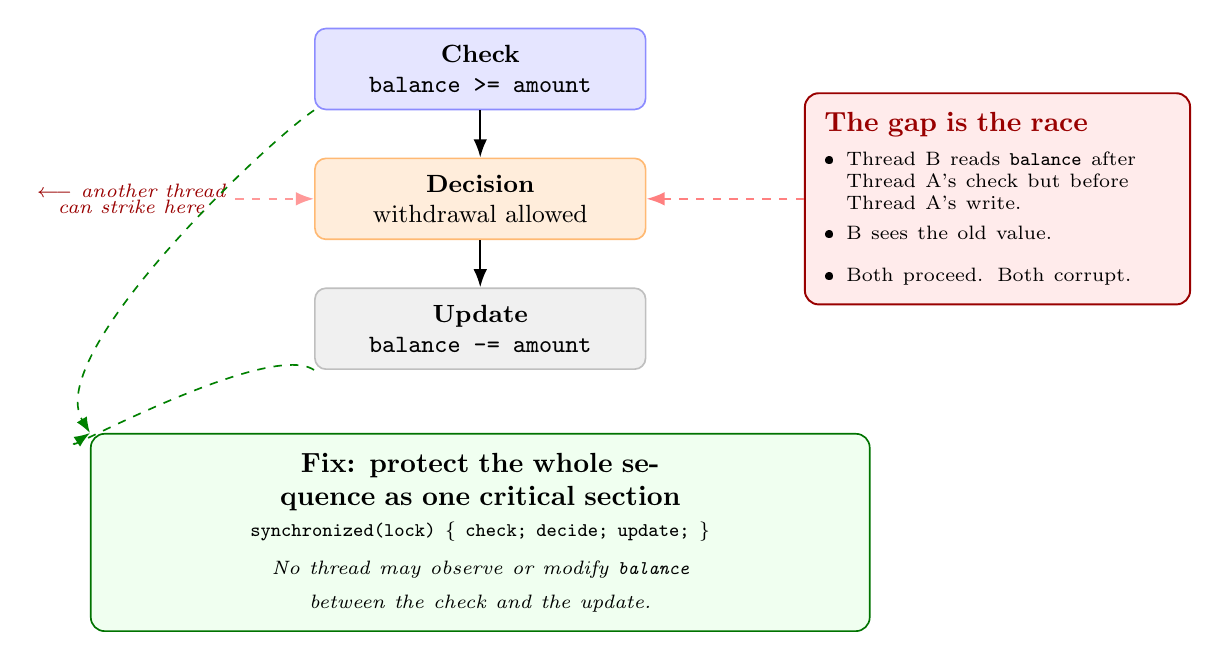
\begin{tikzpicture}[
			stepbox/.style={draw, rounded corners=4pt, align=center,
				inner sep=6pt, font=\small},
			]
			
			%% -- The three-step sequence (left column)
			\node[stepbox, fill=blue!10, draw=blue!45, line width=0.6pt,
			minimum width=4.2cm, minimum height=1.0cm] (c1)
			{\textbf{Check}\\\texttt{balance >= amount}};
			
			\node[stepbox, fill=orange!14, draw=orange!55, line width=0.6pt,
			minimum width=4.2cm, minimum height=1.0cm,
			below=6mm of c1] (c2)
			{\textbf{Decision}\\withdrawal allowed};
			
			\node[stepbox, fill=gray!12, draw=gray!50, line width=0.6pt,
			minimum width=4.2cm, minimum height=1.0cm,
			below=6mm of c2] (c3)
			{\textbf{Update}\\\texttt{balance -= amount}};
			
			\draw[arrow] (c1) -- (c2);
			\draw[arrow] (c2) -- (c3);
			
			%% -- Brace / gap label between check and update
			\node[font=\scriptsize\itshape, text=red!60!black, align=center,
			left=10mm of c2] (gap)
			{$\longleftarrow$ another thread\\[-2pt]can strike here};
			\draw[dashedarrow, red!40] (gap.east) -- (c2.west);
			
			%% -- Danger box (right side)
			\node[draw=red!60!black, fill=red!8, rounded corners=5pt,
			text width=4.4cm, align=left,
			inner sep=7pt, line width=0.7pt,
			right=20mm of c2] (danger)
			{
				\textcolor{red!60!black}{\textbf{The gap is the race}}\\[4pt]
				\scriptsize
				\textbullet\enspace Thread B reads \texttt{balance} after\\
				\hspace{8pt}Thread A's check but before\\
				\hspace{8pt}Thread A's write.\\[3pt]
				\textbullet\enspace B sees the old value.\\[3pt]
				\textbullet\enspace Both proceed. Both corrupt.
			};
			
			\draw[dashedarrow, red!50] (danger.west) -- (c2.east);
			
			%% -- Solution hint (bottom, spanning full width)
			\node[draw=green!45!black, fill=green!6, rounded corners=5pt,
			text width=9.4cm, align=center,
			inner sep=7pt, line width=0.6pt,
			below=8mm of c3] (fix)
			{
				\textbf{Fix: protect the whole sequence as one critical section}\\[3pt]
				\scriptsize
				\texttt{synchronized(lock) \{ check; decide; update; \}}\\[2pt]
				\itshape No thread may observe or modify \texttt{balance} between the check and the update.
			};
			
			\draw[dashedarrow, green!50!black, line width=0.6pt]
			(c1.south west) .. controls +(-6mm,-4mm) and +(-6mm,10mm) .. (fix.north west);
			\draw[dashedarrow, green!50!black, line width=0.6pt]
			(c3.south west) .. controls +(-6mm,4mm) and +(-6mm,-4mm) .. (fix.north west);
			
		\end{tikzpicture}
	\end{center}
	
\end{frame}
	
	% ============================================================
	\begin{frame}[fragile]{Student Repair}
		\begin{lstlisting}[language=Java]
			public synchronized void withdraw(int amount) {
				if (balance >= amount) {
					balance -= amount;
				}
			}
		\end{lstlisting}
		
		\vspace{0.3cm}
		
		\begin{block}{Why this works}
			For an instance method, \texttt{synchronized} uses the monitor of \texttt{this}.
		\end{block}
	\end{frame}
	
	% ============================================================
	\begin{frame}{Why Method-Level Synchronization Works}
		\begin{itemize}
			\item The method is guarded by the instance monitor
			\item Only one thread at a time may execute \texttt{withdraw()} on the same account object
			\item The check and the update are now one atomic critical section
			\item Visibility of the updated balance is guaranteed for subsequent synchronized access
		\end{itemize}
		
		\bigskip
		
		\begin{alertblock}{Important}
			This works only if threads operate on the same account instance.
		\end{alertblock}
	\end{frame}
	
	% ============================================================
	\begin{frame}{Instance Lock vs Static Lock}
		\centering
		\begin{tabular}{@{}lll@{}}
			\toprule
			\textbf{Form} & \textbf{Lock used} & \textbf{Scope} \\
			\midrule
			\texttt{synchronized} instance method & \texttt{this} & one object instance \\
			\texttt{static synchronized} method & \texttt{ClassName.class} & all instances of the class \\
			\bottomrule
		\end{tabular}
		
		\bigskip
		
		\begin{block}{Interpretation}
			Choose the lock scope based on what state is shared:
			shared per object, or shared across all objects.
		\end{block}
	\end{frame}
	
	% ============================================================
	\begin{frame}{Common Pitfalls}
		\begin{itemize}
			\item Using different lock objects for the same shared data
			\item Locking on an object whose identity may change
			\item Assuming synchronized methods make every called method automatically thread-safe
			\item Confusing visibility with atomicity
		\end{itemize}
		
		\bigskip
		
		\begin{alertblock}{Preview}
			A \texttt{volatile} variable can help with visibility, but it does \textbf{not} make compound operations like \texttt{count++} atomic.
		\end{alertblock}
	\end{frame}
	
	% ============================================================
	\begin{frame}{Lab Discussion Prompts}
		\begin{enumerate}
			\item Why is the original \texttt{withdraw()} unsafe?
			\item What makes the repaired version atomic?
			\item What object is actually used as the lock?
			\item When would \texttt{static synchronized} be appropriate instead?
		\end{enumerate}
		
		\bigskip
		
		\begin{alertblock}{Teaching objective}
			Students should connect code syntax to monitor identity and shared-state scope.
		\end{alertblock}
	\end{frame}
	
	% ============================================================
	\begin{frame}{Part 2 Summary}
		\begin{itemize}
			\item \texttt{synchronized} guarantees both mutual exclusion and visibility
			\item Unlock of monitor \(M\) happens-before subsequent lock of \(M\)
			\item A shared lock can eliminate the counter race
			\item The bank-account bug exists because check and update were not atomic together
			\item Method-level synchronization uses the instance monitor
		\end{itemize}
		
		\bigskip
		
		\begin{alertblock}{Bridge forward}
			Next we move from race elimination to deadlock:
			what happens when threads wait on each other’s locks?
		\end{alertblock}
	\end{frame}
	
\end{document}